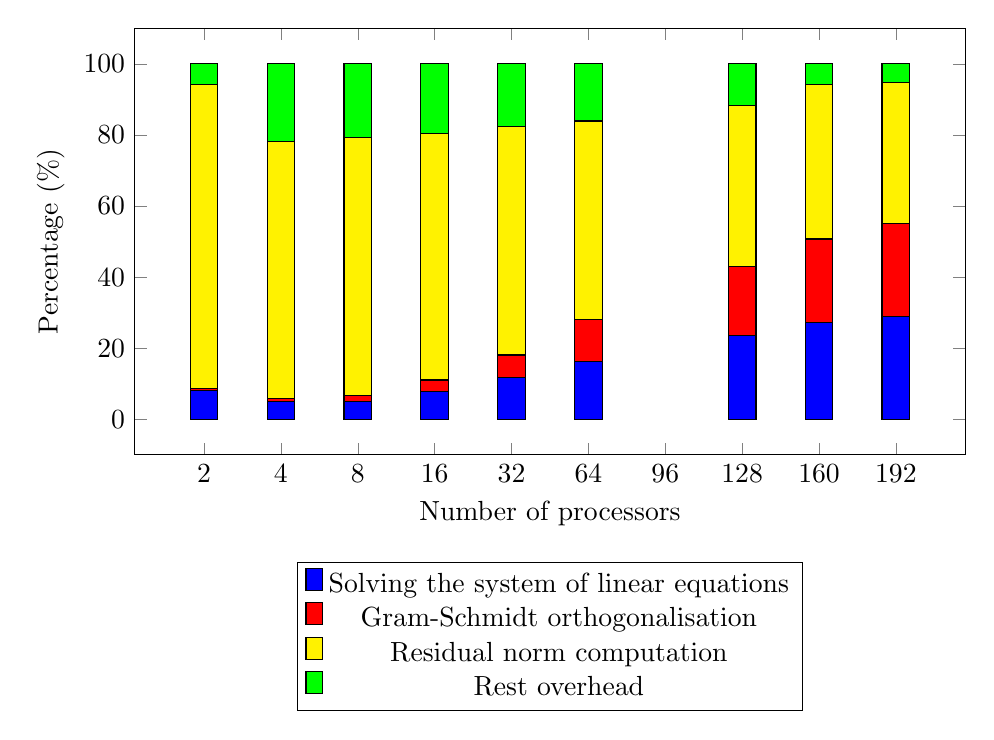
\begin{tikzpicture}
 \begin{axis}[
  ybar stacked,
  height=7cm,
  width=\textwidth,
  xlabel=Number of processors,
  symbolic x coords={2, 4, 8, 16, 32, 64, 96, 128, 160, 192},
  legend style={
   at={(0.5, -0.25)},
   anchor=north
  },
  ylabel={Percentage (\%)}]
  \addplot[ybar, fill=blue] plot coordinates {
   (2, 8.14)
   (4, 5.12)
   (8, 5.04)
   (16, 7.73)
   (32, 11.74)
   (64, 16.38)
   (96, 0)
   (128, 23.48)
   (160, 27.15)
   (192, 28.88)};
  \addplot[ybar, fill=red] plot coordinates {
   (2, 0.46)
   (4, 0.79)
   (8, 1.69)
   (16, 3.32)
   (32, 6.36)
   (64, 11.73)
   (96, 0)
   (128, 19.4)
   (160, 23.57)
   (192, 26.11)};
  \addplot[ybar, fill=yellow] plot coordinates {
   (2, 85.66)
   (4, 72.18)
   (8, 72.53)
   (16, 69.23)
   (32, 64.27)
   (64, 55.8)
   (96, 0)
   (128, 45.44)
   (160, 43.34)
   (192, 39.75)};
  \addplot[ybar, fill=green] plot coordinates {
   (2, 5.74)
   (4, 21.91)
   (8, 20.74)
   (16, 19.72)
   (32, 17.63)
   (64, 16.09)
   (96, 0)
   (128, 11.68)
   (160, 5.93)
   (192, 5.26)};
  \legend{
   Solving the system of linear equations,
   Gram-Schmidt orthogonalisation,
   Residual norm computation,
   Rest overhead}
 \end{axis}
\end{tikzpicture}
